{Given the graph of $f$, identify the intervals of increasing and decreasing as well as the $x$ coordinates of the relative extrema.\\
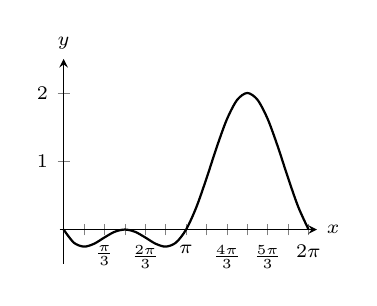
\begin{tikzpicture}
\begin{axis}[width=.4\textwidth,tick label style={font=\scriptsize },
	axis y line=middle,axis x line=middle,
    xtick={0.524,1.047,...,6.5},
	xticklabels={,$\frac\pi3$,,$\frac{2\pi}3$,,$\pi$,,$\frac{4\pi}3$,,$\frac{5\pi}3$,,$2\pi$},
    ymin=-.5,ymax=2.5,
	xmin=-.1,xmax=6.5,name=myplot]
\addplot [{\colorone},smooth,thick,domain=0:6.28] {(sin(deg(x)))^2-sin(deg(x))};
\end{axis}
\node [right] at (myplot.right of origin) {\scriptsize $x$};
\node [above] at (myplot.above origin) {\scriptsize $y$};
\end{tikzpicture}}
{decreasing on $(0,\frac\pi6)\cup(\frac\pi2,\frac{5\pi6})\cup(\frac{3\pi}2,2\pi)$,\\
increasing on $(\frac\pi6,\frac\pi2)\cup(\frac{5\pi}6,\frac{3\pi}2)$;\\
local maxima when $x=\frac\pi2,\frac{3\pi}2$,\\
local minima when $x=\frac\pi6,\frac{5\pi}6$.}
